\subsection{Zeichnen aller Polylines}
\label{sub:zeichnen_aller_polylines}
  Nachdem auf der Karte nun ein einzelner Trip angezeigt und animiert werden kann, sollte nun versucht werden alle Polylines der Trips auf der Karte anzuzeigen. Abbildung \ref{fig:prozess/draw_all_shapes} zeigt, wie dies für das Boston MBTA Feed aussieht.

  \begin{figure}[htbp]
    \begin{center}
      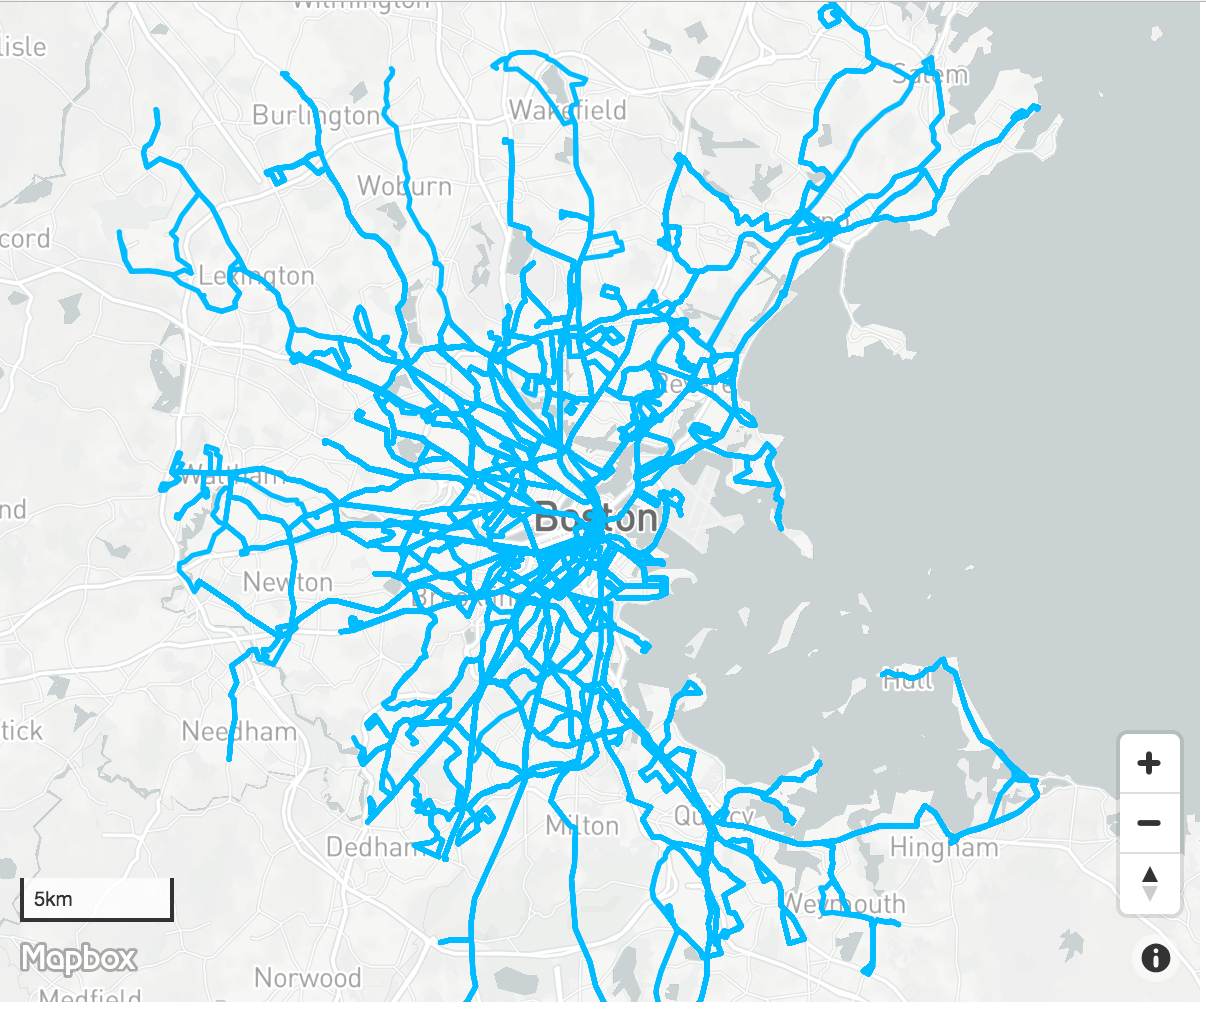
\includegraphics[width=0.5\textwidth]{prozess/draw_all_shapes}
      \caption{Darstellung aller Polylines auf der Karte}
      \label{fig:prozess/draw_all_shapes}
    \end{center}
  \end{figure}
  
  Zwar konnten alle Polylines auf der Karte angezeigt werden, allerdings bei sehr langer Rechen- und Ladezeit. Durch die erhöhung der in der Datenbank abzufragenden Datenmenge, wurden neue Probleme offengelegt. Die ursprüngliche Datenrepräsentation der Polylines in der Datenbank ist nicht optimal und die Daten lassen sich nicht performant genug abfragen. Im folgenden sollen die Optimierungsmaßnahmen, welche an der Polyline und der Datenbank zur Steigerung der Performanz unternommen wurden, aufgezeigt werden.

  \subsubsection{Polyline optimieren}
  \label{ssub:polyline_optimieren}

    Die Optimierung der Polyline ist ein sehr wichtiger Aspekt in meiner Arbeit und soll in diesem Abschnitt vertieft werden. 

    \subsubsection*{Ramer–Douglas–Peucker}
    \label{ssub:ramer_douglas_peucker}
      Das Problem: Die im Stuttgart-VVS Feed zur Verfügung gestellten Polylines sind Überdefiniert und können aus tausenden Punkten bestehen. Für eine Visualisierung ist eine solche Genauigkeit nicht notwendig und aufgrund der großen Datenmenge problematisch. Durch die Verwendung des "`Ramer–Douglas–Peucker"' (RDP) Algorithmus kann die Anzahl der Punkte einer Polyline drastisch reduziert werden. Der Vorteil besteht darin, dass dabei nicht der Linienverlauf verändert wird. Abbildung~\ref{fig:simplify} zeigt ein Beispiel einer solchen Vereinfachung mittels einer JavaScript Bibliothek\footnote{Simplify.js \url{http://mourner.github.io/simplify-js/}}.

      \begin{figure}[htbp]
        \centering
        \subfloat[Polyline vor RDP]{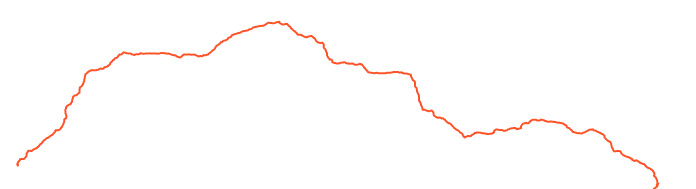
\includegraphics[width=0.48\textwidth]{simplify_before.jpg}\label{fig:simplify_before}}
        \hfill
        \subfloat[Polyline nach RDP]{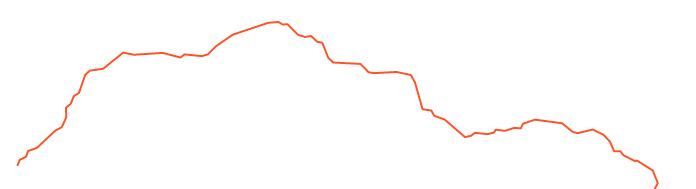
\includegraphics[width=0.48\textwidth]{simplify_after.jpg}\label{fig:simplify_after}}
        \caption{Vereinfachung einer Polyline mittels Simplify.js}
        \label{fig:simplify}
      \end{figure}

      Ausgangspunkt ist eine Polyline mit $\approx1000$ Punkten (\ref{fig:simplify}a). Nach der Vereinfachung (\ref{fig:simplify}b) ist die Anzahl auf 100 Punkte reduziert, ohne dabei visuell merklich einzubüßen. Dies ist eine erhebliche Reduzierung der Punkte um 90\%. Wie wirkt sich dieser Algorithmus positiv auf das Projekt aus? Die Vorteile sind weitreichend. Sehen wir uns die Shape Tabelle in Abbildung \ref{fig:shape_simplify} an. \ref{fig:shape_simplify}a zeigt 394 Reihen vor der Optimierung und nur noch 140 (\ref{fig:shape_simplify}b) nach Anwendung des RDP Algorithmus.

      \begin{figure}[htbp]
        \centering
        \subfloat[Shapte Tabelle vor RDP]{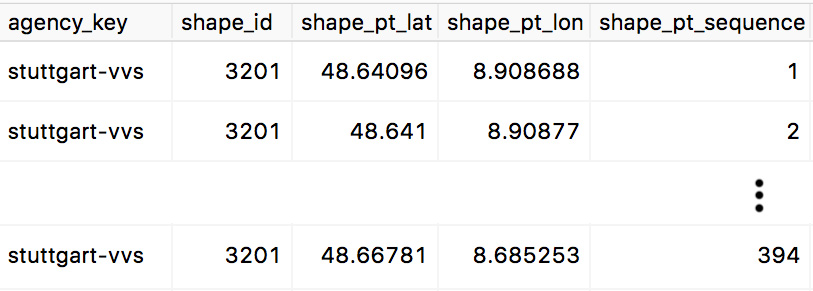
\includegraphics[width=0.48\textwidth]{shape_simplify_before.jpg}\label{fig:shape_simplify_before}}
        \hfill
        \subfloat[Shapte Tabelle nach RDP]{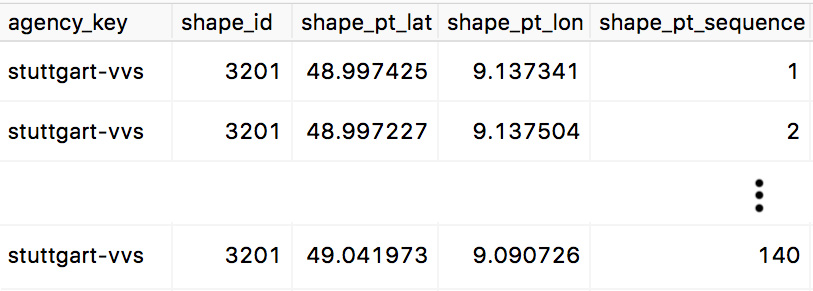
\includegraphics[width=0.48\textwidth]{shape_simplify_after.jpg}\label{fig:shape_simplify_after}}
        \caption{Reduzieren der Polyline via RDP}
        \label{fig:shape_simplify}
      \end{figure}

      In seinem Originalzustand hat das verwendete VVS Feed 1,085,859 Mio Zeilen. Nach der Anwendung sind diese auf 617,653 Tsd. verringert. Testet man folgende PostgreSQL Abfrage
      \colorbox{materialGrey}{\texttt{\color{white}{{\color{materialBlue}SELECT} * {\color{materialBlue}FROM} gtfs\_shapes {\color{materialBlue}WHERE} shape\_id = {\color{materialRed}3201}}}}
      die alle Punkte einer Polyline ausgeben soll, so ergibt sich für ein optimiertes Feed eine Query Zeit von $\approx145 ms$ und für das nicht optimierte Feed $\approx250 ms$. Schon durch diese einfache Methode sind bereits erste Performance Steigerungen wahrnehmbar.\\

      Den RDP Algorithmus habe ich auf das GTFS Feed angewendet, noch bevor die Daten der Polyline in die Datenbank importiert werden. Dadurch muss die Polyline nicht während der Laufzeit vereinfacht werden, sondern diese Rechenzeit kann eingespart werden. In Kapitel \ref{...} wird ein Tool namens \texttt{gtfstidy} vorgestellt, dass GTFS Feeds optimieren kann. Dabei ist auch das vereinfachen von Polylines mittels RDP möglich.

    % subsubsection ramer_douglas_peucker (end)

    \subsubsection*{Aggregieren der Shape Tabelle}
    \label{ssub:aggregieren_der_shape_tabelle}
      In GTFS wird für jeden Punkt einer Polyline eine Reihe in der Datenbank belegt. Diese Abfolge ist durch eine sogenannte \texttt{Shape Point Sequence} festgelegt, was nichts anderes ist als eine Zahl von $1$ bis $n$. Dies ist auch bereits in obiger Tabelle \ref{fig:shape_simplify} zu sehen gewesen. Sehr viel effektiver wäre es allerdings, diese Punkte nicht Reihenweise zu speichern, sondern alle zusammen gehörenden Punkte in nur einem einzigen Feld. Dies ist in PostgreSQL durch eine Aggregierung möglich. Daraus ergibt sich folgende Shape Tabelle:

      \begin{figure}[htbp]
        \begin{center}
          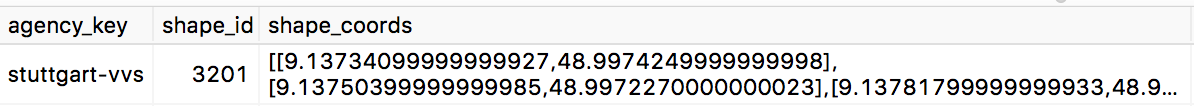
\includegraphics[width=\textwidth]{aggregated.png}
          \caption{Aggregierte Koordinaten der Shape Tabelle}
          \label{fig:aggregated}
        \end{center}
      \end{figure}

      Wie zu sehen ist benötigt nun eine Polyline in der Shape Tabelle nicht mehr 140 Reihen, sondern nur noch eine einzige. Für diese Arbeit ist dies auf alle Polylines angewendet worden und in einer neuen Tabelle namens \texttt{denormalized\_shapes} abgespeichert. Dadurch ist die Berechnung der Aggregierung nur einmal nötig. Der SQL-Befehl dafür ist dem Anhang unter \ref{lst:sql_aggregate_shape}. zu entnehmen.
      Wenden wir die selbe SQL Abfrage, die bereits oben Verwendung fand, auf die neue \texttt{denormalized\_shapes} Tabelle an. Die Query Zeit ist auf $\approx1ms$ gesunken. Anstatt hunderte Reihen muss nur eine einzige Reihe ausgelesen werden, was sehr sehr schnell ist. Durch das Denormalisieren\footnotemark der Shape Tabelle ist auch die Anzahl der Reihen in der Datenbank, auf ein Minimum gesunken. Von den früheren 617,653 Tsd. Reihen, sind durch die Aggregation nur noch 4,524 Tsd. übrig.

      \footnotetext{Denormalisieren beschreibt den Prozess der Relationsauflösung von Datenbanktabellen.}
    
    % subsubsection aggregieren_der_shape_tabelle (end)

    \subsubsection*{Polyline Encoding}
    \label{ssub:polyline_encoding}
      Die letzte Maßnahme zur Optimierung der Polyline stellt das sogenannte Polyline Encoding dar. Wie dieses Verfahren genau funktioniert, geht an dieser Stelle zu weit. Hier soll nur erklärt werden, was unter Polyline Encoding verstanden wird und warum es hier eine Anwendung findet.\\

      Das Polyline Encoding kann in JavaScript beispielsweise durch das Google-Polyline\footnote{\url{https://www.npmjs.com/package/google-polyline}} Paket eingesetzt werden. Das Encoding wandelt eine Polyline, bestehend aus Punkten, in einen String um. Zum Beispiel die Punkte: (38.5, -120.2), (40.7, -120.95), (43.252, -126.453) werden als
      \colorbox{materialGrey}{\texttt{\color{white}{\_p\textasciitilde iF\textasciitilde ps|U\_ulLnnqC\_mqNvxq`@}}}
      codiert. Dies geschieht in meiner Anwendung immer genau dann, bevor Daten von Server in Richtung Client geschickt werden: Encode $\rightarrow$ Send $\rightarrow$ Decode. Da eine codierte Polyline weniger Zeichen benötigt, kann damit Datenvolumen bei der Kommunikation zwischen Server und Client gespart werden.

    % subsubsection polyline_encoding (end)
  % subsubsection polyline_optimieren (end)
% subsection zeichnen_aller_polylines (end)